\chapter{METODOLOGIA}

%Metodologia da bibliografia
\section{Metodologia usada no Levantamento Bibliográfico}

Para atingir os objetivos que orientam este estudo, os procedimentos metodológicos foram planejados tendo como base programas educacionais que visam a promoção do empreendedorismo e comportamento empreendedor na condução dos cursos de graduação, em instituições de ensino públicas e particulares, como também Startups de natureza educacional.


\section{Programa Empreenda AGRO Sustentável: considerações metodológicas}


As atividades serão desenvolvidas por meio de quatro Workshops, que constam metodologias ativas, oficinas, palestras, e ferramentas tecnológicas visando à sinergia entre as estratégias de inovação no uso de tecnologias educacionais e os objetivos da proposta, com vistas a promover aprendizagem significativa e colaborativa. Todas as etapas do projeto de pesquisa serão planejadas e executadas utilizando a metodologias ativas, objetivando o aprendizado do uso das ferramentas de gestão e planejamento de empreendimentos.
Durante os módulos do projeto (Workshops), os participantes testarão de seus projetos para que novas requisições sejam realizadas e/ou que erros nos planejamentos sejam encontrados e, consequentemente, debatidos e mitigados, utilizando para isso os métodos de modelagem de negócio (Lean Canvas e Business Model Canvas). Depois que todas as Sprints (atividades dos três Workshops) forem finalizadas, ou seja, que todos os módulos forem trabalhados, será iniciado um ciclo de Apresentações e desenvolvimento da habilidade de apresentação e demonstração dos produtos por meio de apresentações (\textit{Pitch}). Destaca-se, ainda, que as inovações passiveis de registro intelectual apresentadas nesta pesquisa serão incentivadas a registro e documentação dos direitos.


\newpage
\subsection{Planejamento Pedagógico}

O Programa Empreenda Agro Sustentável trás a proposta do trabalho ao ensino do empreendedorismo de forma multidimensional e  multidisciplinar e disciplinado. Tal programa utilizou-se de Workshops particionados em temas que permitem a compreensão global do empreendedorismo ao mesmo tempo que, admite o ser humano como um ser multidimensional e culturalmente contextualizado no desenvolvimento de um negócio inovador. 

A proposta do programa combina oficinas para o desenvolvimento das características negociais e seus planos com palestras ministradas por profissionais de alto conhecimento nas áreas específicas de um negocio escalável. Com a aprendizagem baseada em equipes \textit{(team-based learning)} o programa delimitou inicialmente a inscrição dos participantes somente em equipes pré-estabelecidas, afim de ter como iniciativa maiores afinidades durante o desenvolvimento dos trabalhos. 


Com a finalidade de propor uma melhor mentoria no desenvolvimento dos objetivos propostos, o programa será desenvolvido em quatro encontros (Workshops), que abordarão temas pertentes ao empreendedorismo e o comportamento empreendedor, a saber:

\begin{itemize}
\item{1\textsuperscript{o} Workshop - O que é Startups, Empreendedorismo, comportamento empreendedor e cultura empreendedora, Problemas (segmentação do mercado), segundo os Objetivos do Desenvolvimento Sustentável (ODS), Modelagem do negócio e Criatividade}

\item{2\textsuperscript{o} Workshop - A busca de oportunidades como Característica Empreendedora, Construção do Lean Canvas, Mapa de Empatia, Validação da Proposta de Valor e Economia colaborativa e Coworking}
\item{3\textsuperscript{o} Workshop -Hackathon: Prototipagem para o MVP, O que você pode fazer por seu cliente e como o cliente adquire seu produto?}

\item{4\textsuperscript{o} Workshop - Pitch e o Demoday}

\end{itemize}


\subsection{1º Workshop}

Buscando um engajamento maior dos participantes Foram
aplicadas cinco estratégias/dinâmicas: Apresentação das ideias propostas inicialmente; Círculo Dourado;
Quem sou eu no Universo?; Descoberta do cliente usuário. Além do
início do desenvolvimento da proposta de valor.

A dinâmica \textbf{"Apresentação das ideias propostas"}\ visa a construção de um panorama visual de todos os insights inscritas no programa, como também as temáticas mais buscadas pelos alunos. As atividades de Expressão Oral (EO) oportunizam aos estudantes a apropriação de recursos linguísticos e interativos inerentes às práticas orais e considerando que a EO pode ser uma eficaz ferramenta para a ensinagem de conteúdos conceituais, procedimentais e atitudinais em contato social \cite{baltar_genero_2010}.

A atividade proposta, leva em consideração que a expressão oral mesmo que incipiente proporcionara aos alunos e todo o grupo o exercício da criticidade, abordar e levantar seus pontos de vista e seus interesses na participação do programa pode executar a sua verve crítica, defender seus pontos de vista ao mesmo tempo que possibilita o aprimoramento das atitudes discursivas da ordem do expor e do argumentar, já que o estudante torna público suas expectativas e se compromete informalmente a comunidade de desenvolver suas propostas. 

Já a segunda dinâmica \textbf{Golden Circle} desenvolvido por \citeonline{sinek_golden_2015} tem por objetivo: criar ou desenvolver o valor de um novo produto, ideia ou negócio, tal dinâmica é pautada em três pilares: O quê, Como e Porquê. O Círculo Dourado e formado por três círculos de diferentes tamanhos que se completam. No certo esta o \textbf{Porquê}, tal círculo objetiva a expressão do real propósito do negócio pensado pelo grupo. Este Refere-se ao conjunto de iniciativas e compromissos pensados para escalar e promover aos usuários e clientes o valor que a Startup realmente acredita. Resumidamente é o que a empresa de fato acredita ser o  diferencial perante a concorrência e ao mercado atual, este é o ponto de partida, principal circulo da dinâmica. 
Nó círculo intermediário está o \textbf{Como}, neste momento o grupo deverá expressar de que forma o empreendimento alcançará seu valor, de forma sucinta este círculo trata do processo tomado pelo grupo objetivando alcançar os clientes e criar o vinculo Cliente/Usuário e o Produto negociável. 
E por fim o círculo maior que contempla o \textbf{O quê}, Neste ponto o desenvolvimento e mais técnico e pragmático, sendo menos emocional, neste ponto o grupo deve explicar de fato o que será o produto promovido aos usuários que alcâncara o valor pensado pela equipe (O porquê), neste momento a liberdade de criação se expressa, em que existe a permissão de pivotar sua ideia inicial para que o produto final esteja de acordo com o valor do negócio, na figura \ref{figura_2} é possível observar o modelo utilizado na dinâmica do Programa.


\begin{figure}[h!]
\centering
\caption{\textbf{Golden Circle}}
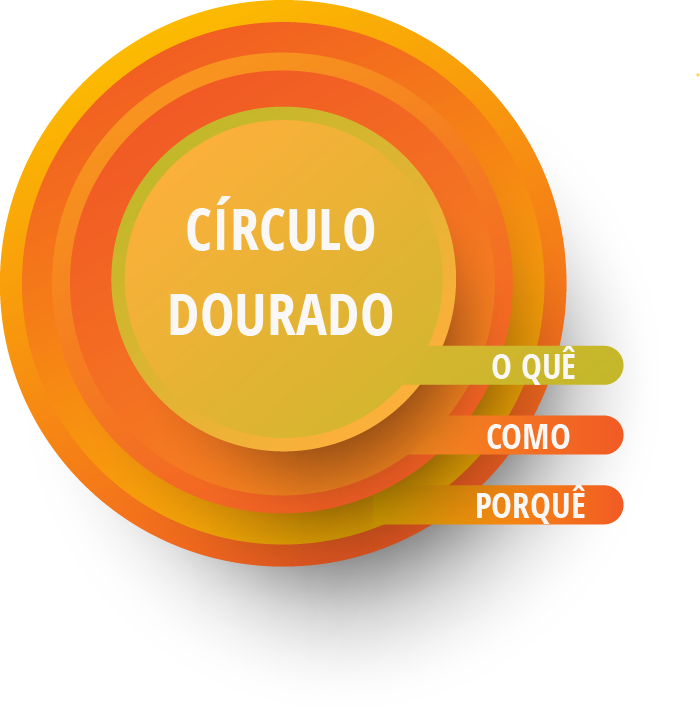
\includegraphics[scale=0.05]{Imagens/circulo_dourado.png}
\fonte{Adaptado de \cite{sinek_golden_2015}}
\label{figura_2}
\end{figure}

\newpage


\subsection{2º Workshop}

CONTINUAR

\subsection{Mobilização das equipes:}

Inicialmente serão abertas vagas para estudantes do curso de graduação ligadas aos cursos de Ciências Agrárias da Universidade Federal de Sergipe-UFS, onde as inscrições serão realizadas por equipe, desde que preencham os seguintes critérios:

	
\begin{itemize}
\item{Estarem regularmente matriculados e cursando quaisquer dos cursos e ao menos um aluno ligado as ciências agrárias;}
\item{Comprovarem disponibilidade de tempo para participação em todas as oficinas programadas;}
\item{Lidar com trabalhos em equipe.}
\end{itemize}

Objetiva-se o alcance de \textbf{120 alunos} participantes efetivos no programa, o qual será considerado o número de amostra para o estudo. 

\newpage



\section{Questionário para análise de Campo}

A utilização de um método de pesquisa em uma dissertação depende da escolha de um modelo mais adequado ao problema da pesquisa e os objetivos pretendidos.

Desta forma esta pesquisa será desenvolvida com caráter descritivo tendo como base o método de pesquisa \textit{Survey} descritivo, uma vez que este método busca contribui para o conhecimento geral de uma área particular de interesse, pois envolve uma coleção de informações de indivíduos por meio de questionários e entrevistas sobre suas atividades ou sobre si mesmos \cite{forza_survey_2002}, como também diversos estudos sobre o empreendedorismo na América Latina têm utilizado \textit{Surveys} realizados em residências ou com apelo direto aos donos de empresas para a coleta de dados, assim como em meios acadêmicos \cite{lima_ser_2015}. 


Assim, esta pesquisa utilizará de um Survey descritivo para analisar o potencial do comportamento empreendedor e a competências Empreendedoras, dos acadêmicos dos cursos de graduação em Ciências Agrárias inscritos no Programa Empreenda AGRO Sustentável, utilizando como fator indutor para melhoria o programa de extensão Empreenda Agro Sustentável a partir do modelo \textit{Global University Entrepreneurial Spirit Students’ Survey} (GUESSS), conhecido nacionalmente por Estudo GUESSS. Esta ferramenta de estudo busca caracterizar o espírito, as atividades e as intenções empreendedores de estudantes universitários, de todos os níveis de estudo e em todos os cursos universitários, bem como as condições de ensino e apoio a atividades empreendedoras. 



Por critérios éticos o questionário aplicado nesta pesquisa atende os termos das Resolução n. 466 de 12 de dezembro de 2012 do Conselho Nacional de Saúde \cite{cns_resolucao_2012}, o qual por se tratar de pesquisa com seres humanos foi submetido ao Comitê de Ética em Pesquisa Envolvendo Seres Humanos (\textbf{CEP}) e a Comissão Nacional de Ética em Pesquisa (\textbf{Conep}) por meio da plataforma Brasil Saúde sendo \textbf{APROVADO} sob o número do Certificado de Apresentação para Apreciação Ética \textbf{CAAE: 23853219.4.0000.5546}. O questionário apresenta 5 conjuntos de questões dos mais diversos contextos relacionados ao empreendedorismo, medindo diferentes elementos do empreendedorismo e comportamento empreendedor no meio educacional tanto vindo dos discentes quanto dos docentes. Destaca-se que o instrumento de pesquisa que será utilizado neste experimento foi composto por Cinco blocos de questões de múltipla escolha baseadas principalmente em escalas de cinco ou sete possibilidades. 

O primeiro conjunto de questões está relacionado a informações que buscam traçar o perfil dos alunos entrevistados, tais como: gênero, faixa etária, curso vinculado e o perfil de interesse nas áreas de estudo ligadas ao empreendedorismo sustentável tal questionário foi baseado no trabalho desenvolvido por \citeonline{lima_educacao_2014}. 

O segundo bloco e composto por 10 questões relacionadas a auto eficácia dos estudantes de múltipla escolha partindo da alternativa “Completamente Inseguro” a Completamente Seguro”. 

O terceiro bloco e composto por 7 questões que analisam a intenção empreendedora do aluno da quais segue uma proporção partindo da resposta, tendo como alternativas partido do “Discordo totalmente” a “Concordo totalmente”.

O Quarto bloco retrata a intenção em ter sua própria empresa ou ser autônomo e por fim o Quinto bloco contendo 11 questões abordará a ligação da família e o apoio familiar no empreendedorismo, tendo como alternativas partido do “Discordo totalmente” a “Concordo totalmente”. 

O universo desta pesquisa é composto por 1.453 discentes dos cursos de graduação nas áreas de agrárias da Universidade Federal de Sergipe (UFS): Engenharia Agronômica, Engenharia Agrícola, Zootecnia, Engenharia Florestal, Medicina Veterinária e Engenharia de Pesca, dados contidos no relatório estatístico de matriculas 2017 da instituição, \cite{campelo_ufs_2018}. É importante levar em conta que este estudo não levou em consideração classe social local de estudo anterior, e desempenho acadêmico do aluno durante a graduação. 
A amostra compreenderá 120 discentes que participarem do Programa Empreenda Agro Sustentável que responderão os questionários instrumento de pesquisa que serão aplicados durante os Workshops. Tais Workshops ocorrerão nos meses de agosto, outubro e novembro de 2019. Tal instrumento será aplicado presencialmente. O estudo caracteriza-se como uma pesquisa de levantamento ou \textit{Survey} do tipo Descritivo sob corte Longitudinal, que segundo \citeonline{tormen_potencial_2005} destaca-se por compreender uma amostra expressiva em relação ao universo pesquisado. Na Figura \ref{figura_1} é possível compreender as fases da tendo como critério a pesquisa tipo \textit{Survey}.

\begin{figure}[!htb]
\centering
\caption{\textbf{Fases da pesquisa tipo Survey}}
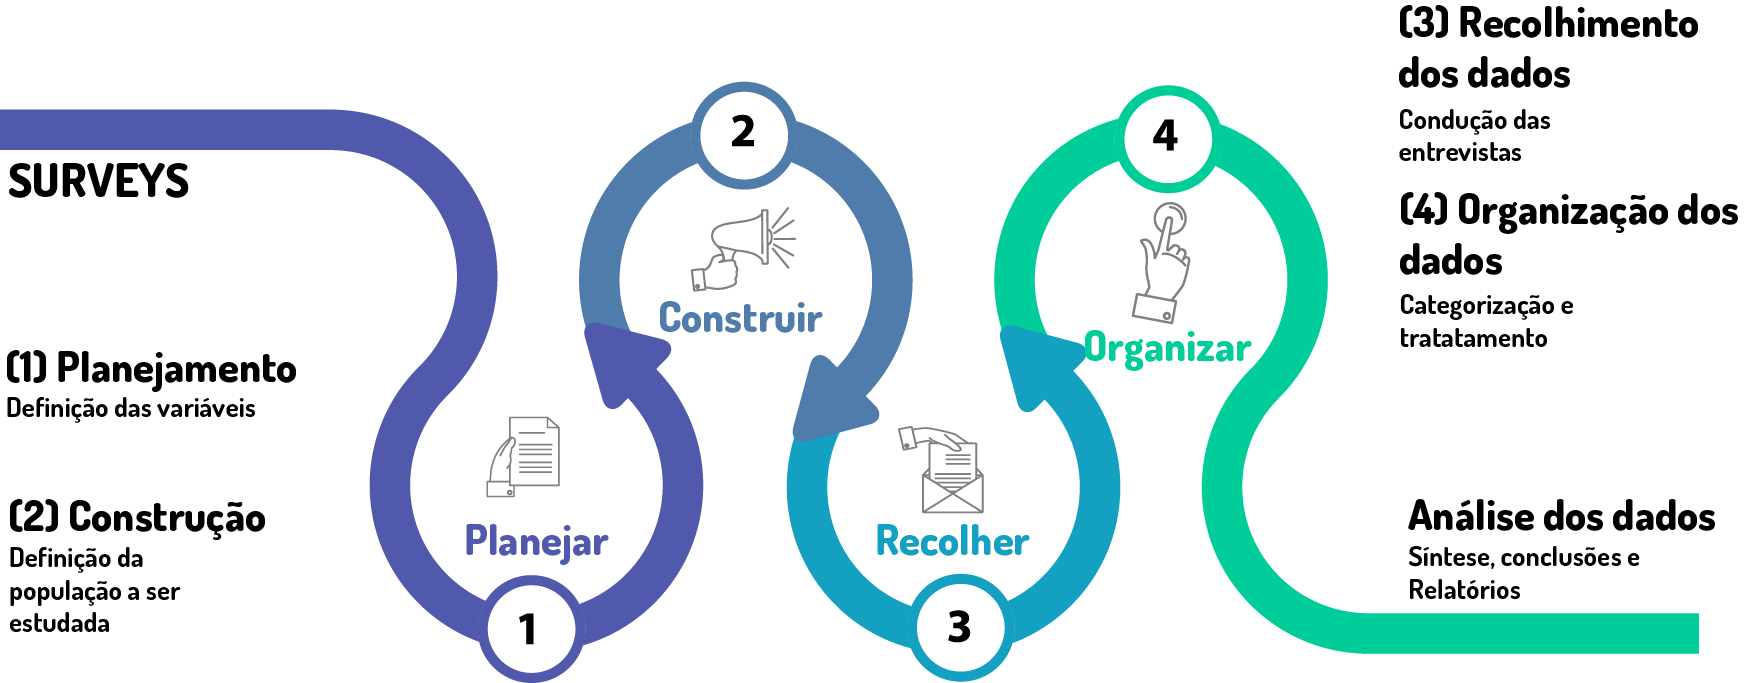
\includegraphics[scale=0.3]{Imagens/diagrama_survey.png}
\fonte{Adaptado de \cite{moser_survey_2017}}
\label{figura_1}
\end{figure}

\clearpage


%estatística
\section{Análises Estatísticas}


Os dados serão tratados, inicialmente, por uma análise de distribuição por meio do teste de
Kolmogorov-Smirnov (p > 0,05). 

Tendo as informações das distribuições dos dados será utilizado uma análise fatorial e análise de variância multivariada buscando aglutinar as variáveis de cada questão em fatores.Tais fatores serão preparadas com o uso da análise fatorial exploratória (AFE) por meio do teste de Bartlett com a significância tendo o p < 0,05, este teste tem o objetivo de aglutinar em fatores únicos os dados obtidos com diferentes itens de escala do questionário \cite{hair_multivariate_2006}. O fatores aglutinados desta pesquisa estão relacionadas aos seguintes fatores:


\begin{itemize}
\item {Interesse em conteúdos relacionados a educação empreendedora;}
\item {Dimensão da Autoeficácia dos estudantes;}
\item {Dimensão da  Intenção empreendedora dos estudantes;}
\item {Dimensão da participação familiar no desenvolvimento empreendedorismo;}
\end{itemize}


Para analisar o desenvolvimento do comportamento empreendedor e os dados correlacionados a este estudo após a participação no programa, será utilizado uma Análise de Variância Multivariada (MANOVA) caso os dados satisfaçam as exigências para tal teste. A MANOVA é uma técnica estatística que analisa independentemente grupos distintos de amostras buscando avaliar as diferenças entre as medias por grupos. A MANOVA tem por objetivo verificar diferenças de grupos de variáveis categóricas (independentes) quanto aos seus impactos sobre diversas variáveis métricas (dependentes) em paralelo  \cite{hair_alise_2009}. 
Este teste aplica-se a esta pesquisa pois ela tem por objetivo avaliar as alterações quanto ao perfil empreendedor em grupos de alunos participantes do Programa de extensão Empreenda Agro Sustentável. Desse modo, é possível avaliar se as diferenças entre os níveis médios dos grupos captados pela \textit{}{survey} são significativas entre os grupos e dentro dos grupos \cite{rocha_avaliacao_2014}. 

A hipótese nula aqui apresentada será utilizada para condução deste experimento. Com a rejeição desta, a hipótese alternativa é comprovada \ \cite{hair_alise_2009}.

\textbf{H0:} Não há diferença entre as médias das medidas que averíguam o perfil empreendedor entre os alunos participantes do Programa de extensão Empreenda Agro Sustentável.

 O processamento dos dados será utilizado o Software Rstudio \cite{rstudio_team_rstudio:_2015}. 


\chapter{RESULTADOS E DISCUSSÃO }
